% \usepackage{xcolor}
% \usepackage[hang, flushmargin]{footmisc}
% \usepackage[
% colorlinks=false, % don't highlight links in color
% linkbordercolor=green, % set border color for internal links
% citebordercolor=green, % set border color for citations
% filebordercolor=magenta, % set border color for file links
% urlbordercolor=cyan, % set border color for URLs
% pdfborder={0 0 1}, % determine border around links
% linkcolor=black,
% citecolor=black,
% filecolor=black,
% urlcolor=black,
% ]{hyperref}
% \usepackage{footnotebackref}

% \usepackage{cite}
% \usepackage{amsmath,amssymb,amsfonts}
% \usepackage{algorithmic}
% \usepackage{graphicx}
% \usepackage{textcomp}

% \def\BibTeX{{\rm B\kern-.05em{\sc i\kern-.025em b}\kern-.08em
%     T\kern-.1667em\lower.7ex\hbox{E}\kern-.125emX}}

% \usepackage[english]{babel}
% \addto\extrasenglish{  
%     \def\figureautorefname{Figure}
%     \def\tableautorefname{Table}
%     \def\algorithmautorefname{Algorithm}
%     \def\sectionautorefname{Section}
%     \def\subsectionautorefname{Subsection}
% }

% \newcommand{\supertiny}{\fontsize{1}{2}\selectfont}

% \usepackage{catoptions}
% \makeatletter

% \def\Autoref#1{%
%   \begingroup
%   \edef\reserved@a{\cpttrimspaces{#1}}%
%   \ifcsndefTF{r@#1}{%
%     \xaftercsname{\expandafter\testreftype\@fourthoffive}
%       {r@\reserved@a}.\\{#1}%
%   }{%
%     \ref{#1}%
%   }%
%   \endgroup
% }
% \def\testreftype#1.#2\\#3{%
%   \ifcsndefTF{#1autorefname}{%
%     \def\reserved@a##1##2\@nil{%
%       \uppercase{\def\ref@name{##1}}%
%       \csn@edef{#1autorefname}{\ref@name##2}%
%       \autoref{#3}%
%     }%
%     \reserved@a#1\@nil
%   }{%
%     \autoref{#3}%
%   }%
% }
% \makeatother

% \usepackage[T1]{fontenc}
% \usepackage{graphicx}
% %\usepackage{color}
% %\renewcommand\UrlFont{\color{blue}\rmfamily}

% \usepackage{amsmath,amssymb,amsfonts}
% \usepackage[inline, shortlabels]{enumitem}
% \usepackage{tabularx}
% \usepackage{caption}
% \usepackage{listings}
% % \usepackage{titlesec}
% \usepackage{ragged2e}

% \usepackage{xurl}
% % \usepackage[hyphens]{url}
% \usepackage{pifont}
% \usepackage{multirow}
% \usepackage[linesnumbered,ruled,vlined]{algorithm2e}
% \usepackage{float}
% \usepackage{listings}
% \usepackage{xcolor}

% \definecolor{codegreen}{rgb}{0,0.6,0}
% \definecolor{codegray}{rgb}{0.5,0.5,0.5}
% \definecolor{codepurple}{rgb}{0.58,0,0.82}
% \definecolor{backcolour}{rgb}{0.95,0.95,0.92}

% \lstdefinestyle{mystyle}{
%     backgroundcolor=\color{backcolour},   
%     commentstyle=\color{codegreen},
%     keywordstyle=\color{magenta},
%     numberstyle=\tiny\color{codegray},
%     stringstyle=\color{codepurple},
%     basicstyle=\footnotesize,
%     breakatwhitespace=false,         
%     breaklines=true,                 
%     captionpos=b,                    
%     keepspaces=true,                 
%     numbers=left,                    
%     numbersep=5pt,                  
%     showspaces=false,                
%     showstringspaces=false,
%     showtabs=false,                  
%     tabsize=2
% }

% \lstset{style=mystyle}

% % --- Tickz
% \usepackage{physics}
% \usepackage{amsmath}
% \usepackage{tikz}
% \usepackage{mathdots}
% \usepackage{yhmath}
% \usepackage{cancel}
% \usepackage{color}
% \usepackage{siunitx}
% \usepackage{array}
% \usepackage{multirow}
% \usepackage{amssymb}
% \usepackage{gensymb}
% \usepackage{tabularx}
% \usepackage{extarrows}
% \usepackage{booktabs}
% \usetikzlibrary{fadings}
% \usetikzlibrary{patterns}
% \usetikzlibrary{shadows.blur}
% \usetikzlibrary{shapes}

% % ---------
% % \usepackage{titlesec}
% \usepackage{pdfpages}
% \usepackage{booktabs}
% \usepackage{csquotes}
% \usepackage{lipsum}  
% \usepackage{arydshln}
% \usepackage{smartdiagram}
% \usepackage{textcomp}
% \usepackage{tabularray}\UseTblrLibrary{varwidth}
% \usepackage{xcolor}
% \def\BibTeX{{\rm B\kern-.05em{\sc i\kern-.025em b}\kern-.08em
%     T\kern-.1667em\lower.7ex\hbox{E}\kern-.125emX}}
% \usepackage{cite}
% \usepackage{amsmath}
% \newcommand{\probP}{\text{I\kern-0.15em P}}
% \usepackage{etoolbox}
% \patchcmd{\thebibliography}{\section*{\refname}}{}{}{}

% \setlength\tabcolsep{0.5pt}

% \newcommand{\before}[1]{\textcolor{red}{#1}}
% \newcommand{\after}[1]{\textcolor{green}{#1}}

% \newcommand{\old}[1]{\textcolor{orange}{#1}}
% \newcommand{\rem}[1]{\textcolor{red}{#1}}
% \newcommand{\todo}[1]{\textcolor{orange}{\newline \textit{\textbf{TODO:} #1}} \newline \newline }



% \newcounter{relation}
% \setcounter{relation}{0}
% \renewcommand{\therelation}{\arabic{relation}}
% \newcommand{\relationautorefname}{Relation}

% \newenvironment{relation}[1][]{%
%     \refstepcounter{relation}%
%     \noindent \raggedright \textit{\textbf{Relation. \therelation}} \hfill$}
% {%
% $ \hfill \phantom{x}

% }

% ====================================================

\section{Introduction}
\label{sec:introduction}

\textit{Les agents autonomes intelligents de cyberdéfense}~\cite{Kott2023} (AICA) sont des agents destinés à être déployés dans des environnements réseau afin de détecter, d'identifier et de caractériser les anomalies/attaques, de développer des contre-mesures et de les exécuter
%
\footnote{
    Théorisés par le \textit{Groupe de travail international AICA} (cf. \url{https://www.aica-iwg.org/}) et basés sur les résultats du \textit{Groupe de travail de recherche IST-152} de l'OTAN.
}.
Les recherches connexes de l'AICA soulignent le besoin croissant d'une \textit{cyberdéfense autonome} pour protéger les environnements décentralisés où les approches centralisées traditionnelles sont inefficaces, comme dans les systèmes basés sur l'IoT. Un système multi-agents (MAS) offre des mécanismes de défense robustes et adaptatifs en décomposant la complexité de la cyberdéfense en sous-tâches déléguées à des agents collaboratifs déployés dans tout le système.

L'approche descendante consiste à concevoir des MAS de cyberdéfense à partir d'architectures et de fonctionnalités prédéfinies. L'\textit{architecture de référence MAS centrée sur l'AICA} (MASCARA)~\cite{Kott2023} décrit un MAS de type AICA avec des composants qui permettent des mécanismes collaboratifs basés sur des plans ou des processus explicitement définis. Cependant, cette approche peut être coûteuse car elle nécessite une connaissance approfondie de l'environnement de déploiement, qui doit être régulièrement mise à jour en raison de changements fréquents, tels que des modifications de topologie ou de nouvelles vulnérabilités.

L'approche ascendante peut inclure l'apprentissage par renforcement multi-agents (MARL)~\cite{Albrecht2024}, où les agents apprennent à atteindre les objectifs de cyberdéfense de manière autonome, renforçant ainsi l'autonomie du MAS~\cite{hammar_stadle4_noms_23}. Malgré des résultats de simulation prometteurs, cette approche ne offre pas les garanties de sécurité nécessaires pour des applications dans le monde réel et ne fournit pas de moyens explicites pour justifier le succès ou l'échec des MAS~\cite{dulacarnold2019}. Ces problèmes entravent le développement de MAS de cyberdéfense entièrement ou semi-autonomes, tels que l'AICA, dans des environnements critiques, où les actions doivent être justifiées compte tenu de leurs conséquences potentiellement irréversibles.

Pour répondre à cette préoccupation, nous proposons de combiner ces deux points de vue en étendant la \textit{relation partielle entre l'historique des agents et le modèle organisationnel}~\cite{soule2024} (PRAHOM). PRAHOM est une approche générale qui permet d'intégrer le modèle organisationnel $\mathcal{M}OISE^+$ dans le cadre MARL, jetant ainsi les bases pour contraindre l'apprentissage. Cependant, cette perspective reste limitée dans sa mise en œuvre et se heurte à des problèmes d'évolutivité avec le nombre de spécifications organisationnelles, ce qui limite son application dans des environnements réseau complexes.

La principale contribution de cet article est le \textit{PRAHOM orienté cyberdéfense} (CoPRAHOM), inspiré du PRAHOM et des travaux connexes. Cet algorithme est spécifiquement destiné à traiter les scénarios de cyberdéfense s'appuyant sur des architectures générales de cyberdéfense telles que MASCARA. Cet algorithme permet aux utilisateurs de contraindre les agents à des rôles et des missions de cyberdéfense. Nous avons mis en œuvre des moyens pratiques pour appliquer CoPRAHOM, également dans le but de répondre aux préoccupations en matière d'évolutivité. L'un des principaux intérêts est d'assurer des garanties de sécurité en intégrant des connaissances spécifiques au domaine, telles que des règles, ou en accélérant ou stabilisant la formation en limitant l'espace de recherche.

Nous avons évalué CoPRAHOM dans le scénario simulé fourni par le 3e défi CAGE~\cite{cage_challenge_3_announcement}. Il s'agit de créer un MAS de cyberdéfense pour détecter, atténuer et éliminer les programmes malveillants dans un essaim de drones. À l'aide de CoPRAHOM, nous avons développé plusieurs modèles de MAS de cyberdéfense. Ces modèles sont utilisés par CoPRAHOM pour guider et contraindre l'entraînement des agents afin de mieux atteindre les objectifs du scénario et de garantir les exigences de sécurité. Nous vérifions que les agents entraînés présentent les stratégies collectives attendues tout en étant affinés tout au long de l'entraînement, ce qui rend le score global comparable à celui des meilleures entrées du classement.

Le reste de cet article est organisé comme suit. \autoref{sec:marl_background} présente les principes fondamentaux du MARL. \autoref{sec:related_works} passe en revue les travaux connexes sur le MARL pour la cyberdéfense et la surveillance de la formation des agents. \autoref{sec:marl_moise_linking} décrit le modèle $\mathcal{M}OISE^+$ et son intégration avec le MARL. \autoref{sec:coprahom} récapitule l'architecture MASCARA que nous avons utilisée conjointement avec l'algorithme CoPRAHOM et discute de sa mise en œuvre. \autoref{sec:experimental_setup} couvre la configuration expérimentale du 3e défi CAGE ainsi que les mesures et critères d'évaluation de CoPRAHOM. \autoref{sec:results_and_discussion} présente et discute les résultats bruts. Enfin, \autoref{sec:conclusion} conclut l'article et présente les orientations futures de la recherche.


\section{Contexte MARL}\label{sec:marl_background}

L'apprentissage par renforcement multi-agents (MARL) étend les principes de l'apprentissage par renforcement (RL) à des scénarios impliquant plusieurs agents en interaction. Les agents visent à maximiser la récompense cumulative globale par l'apprentissage, mais la présence d'autres agents introduit une complexité supplémentaire en raison de la nature dynamique de l'environnement.

Le MARL est souvent modélisé à l'aide du processus de décision markovien décentralisé partiellement observable (Dec-POMDP)~\cite{Beynier2013}, un cadre adapté aux environnements où les agents ont des observations limitées et différentes. Un Dec-POMDP est formellement défini comme un tuple $(S, \{A_i\}, T, R, \{\Omega_i\}, O, \gamma)$ :

\begin{itemize}
    \item $S$ : ensemble fini d'états décrivant l'environnement.
    \item $\{A_i\}$ : un ensemble d'ensembles d'actions, un pour chaque agent $i$.
    \item $T$ : La fonction de probabilité de transition d'état $T(s, \vec{a}, s') = P(s'|s, \vec{a})$, où $\vec{a}$ est l'action conjointe de tous les agents.
    \item $R$ : la fonction de récompense $R(s, \vec{a}, s')$, qui associe les états et les actions à une récompense.
    \item $\{\Omega_i\}$ : ensemble d'ensembles d'observations, un pour chaque agent $i$.
    \item $O$ : La fonction de probabilité d'observation $O(\vec{o} | s', \vec{a})$, où $\vec{o}$ est l'observation conjointe de tous les agents.
    \item $\gamma \in [0,1]$ : Le facteur d'actualisation pour les récompenses futures.
\end{itemize}

Dans MARL, chaque agent $i$ maintient une politique $\pi_i: H \times \Omega \rightarrow A$, qui mappe une action $a \in A$ à partir d'une observation $\omega \in \Omega$ et, éventuellement, de l'historique de l'agent $h \in H, h=\langle(\omega_0,a_0),(\omega_1,a_1)\dots(\omega_{n_e},a_{n_e})\rangle$ (avec $n_e \in \mathbb{N}$, le nombre d'étapes par épisode). Une politique conjointe $\pi_{\text{joint}} = (\pi_1, \pi_2, \ldots, \pi_n)$ décrit le comportement collectif de tous les agents.

L'objectif final est de trouver une politique conjointe $\pi_{\text{joint}}$ qui maximise la récompense cumulative attendue $U(\pi^*_{\text{joint}}) = \mathbb{E}\left[\sum_{t=0}^{\infty} \gamma^t R(s_t, \vec{a}_t)\right]$. Au lieu de viser uniquement un optimum global, notre approche met l'accent sur l'obtention de solutions approximatives avec une récompense suffisante.

Diverses méthodes ont été proposées pour relever les défis posés par les MARL.
%
\textbf{Les méthodes basées sur la valeur}, telles que QMIX~\cite{rashid2018}, estiment la fonction de valeur $Q(s,\vec{a})$, qui représente la récompense cumulative attendue pour un état donné $s$ et une action conjointe $\vec{a}$. Si ces méthodes ont donné des résultats prometteurs dans des scénarios simples, elles ont souvent du mal à exploiter efficacement la communication multi-agents pour améliorer les récompenses globales~\cite{oroojlooy2021review}.
%
\textbf{Les méthodes basées sur les politiques}, notamment l'optimisation de la politique proximale multi-agents (MAPPO)\cite{yu2022surprising} et le gradient de politique déterministe profond multi-agents (MADDPG)\cite{lowe2017multi}, paramètrent directement la politique sous la forme $\pi_\theta$ et l'optimisent, en utilisant éventuellement un entraînement centralisé avec une exécution décentralisée. Nous avons privilégié ces méthodes car elles ont démontré une efficacité significative dans divers contextes coopératifs et compétitifs à agents multiples~\cite{yu2022surprising}\cite{lowe2017multi}.
%
Enfin, les méthodes \textbf{Actor-Critic} combinent les approches basées sur la valeur et celles basées sur la politique. Par exemple, dans COMA (Counterfactual Multi-Agent Policy Gradients), l'acteur met à jour les paramètres de la politique dans la direction indiquée par le critique, qui évalue la politique actuelle. Bien que ces méthodes se soient révélées efficaces dans des configurations à agent unique, des efforts supplémentaires sont nécessaires pour les adapter pleinement à des scénarios multi-agents, en particulier pour gérer la complexité introduite par l'influence mutuelle des agents~\cite{papoudakis2021agent}.


\section{Travaux connexes}
\label{sec:related_works}

Nous définissons le MARL orienté organisation comme le vaste domaine de recherche englobant les études qui introduisent des spécifications explicites (telles que des règles, des rôles ou des protocoles) afin de guider ou de restreindre le processus de formation MARL pour répondre à des exigences. Bien que l'intégration explicite de spécifications organisationnelles dans le MARL ne soit pas largement traitée dans la littérature, plusieurs approches ont été proposées pour intégrer certaines contraintes dans les MAS afin de garantir que les agents se conforment à des exigences spécifiques.

\textbf{Apprentissage avec des contraintes organisationnelles} \quad
Dans \cite{cruz2020norms}, les auteurs présentent une méthode pour intégrer des normes dans les algorithmes d'apprentissage des agents, garantissant ainsi que leur comportement reste dans des limites acceptables. De plus, \cite{villatoro2011social} propose un mécanisme permettant aux agents d'apprendre et de s'adapter aux normes sociales dans des environnements dynamiques, soulignant l'importance de l'adaptation aux normes dans les MAS.
%
Un sous-ensemble pertinent de travaux appartient au domaine de l'apprentissage par renforcement guidé par des spécifications, qui vise à générer des politiques permettant d'accomplir des tâches spécifiques à l'aide de spécifications externes pour guider l'apprentissage dans la réalisation d'objectifs soumis à des contraintes données~\cite{Bansal2022}. Jothimurugan et al.~\cite{Jothimurugan2021} proposent l'apprentissage de spécifications logiques, exploitant la structure compositionnelle des spécifications pour générer des politiques pour des tâches complexes. Cependant, cela ne s'inscrit pas complètement dans le cadre MARL que nous avons défini, car cela nécessite l'introduction de spécifications logiques.

\textbf{MARL dans la cybersécurité et les opérations cyberautonomes} \quad
Le MARL a également été appliqué à la cybersécurité afin de développer des systèmes autonomes capables de se défendre contre les cybermenaces. Albrecht et al.~\cite{Albrecht2024} explorent l'utilisation du MARL pour former des agents dans des environnements dynamiques afin d'atteindre des objectifs de cybersécurité.
Comme indiqué précédemment dans Kott et al.~\cite{Kott2023}, certains travaux impliquant les AICA comprennent le développement de cadres de simulation pour la formation sur mesure d'agents autonomes dans un environnement décentralisé~\cite{Drasar2020}.
De même, dans \cite{Hammar2022}, les auteurs présentent un cadre utilisant des méthodes d'identification de systèmes pour intégrer des jumeaux numériques à MARL afin d'améliorer l'automatisation de la cybersécurité et l'applicabilité de MARL dans des systèmes réels.

\textbf{Approches basées sur des politiques} \quad
Certains travaux liés aux approches basées sur des politiques favorisent des moyens de faire respecter les contraintes organisationnelles en définissant des politiques explicites qui régissent le comportement des agents. Dans \cite{krupanski2015norm}, l'utilisation de politiques normatives est étudiée pour guider les interactions entre agents et les processus décisionnels. De plus, \cite{vos2020governing} explore l'utilisation de mécanismes de gouvernance pour faire respecter les politiques organisationnelles dans les systèmes décentralisés. Cependant, ces approches se heurtent à un manque de praticité dans leur utilisation et peuvent être difficiles à expliquer, car la plupart des politiques sont opaques et ne peuvent pas être facilement modifiées.

\textbf{Cadres intégrant les aspects organisationnels} \quad
Wang et al.~\cite{Wang2020} introduisent une approche dans laquelle des rôles émergents similaires sont encouragés à se spécialiser conjointement dans des tâches spécifiques. Tosic et al.~\cite{Tosic2010} proposent un cadre de coordination basé sur les capacités de communication des systèmes multi-agents. Zheng et al.~\cite{Zheng2018} présentent une plateforme pour le MARL qui vise à faciliter la recherche sur l'intelligence collective artificielle en fournissant un ensemble complet de mesures d'évaluation permettant de comparer les performances des algorithmes MARL. Cependant, elle ne tient pas compte des spécifications susceptibles d'inciter les agents à adhérer à un comportement attendu, tel que des missions.


Malgré ces avancées, les recherches utilisant explicitement des spécifications organisationnelles pour contraindre l'apprentissage des agents en fonction des exigences sont encore rares. À notre connaissance, aucun travail existant ne facilite la génération d'un MAS qui satisfait explicitement des contraintes organisationnelles supplémentaires. L'originalité de CoPRAHOM réside dans l'utilisation explicite d'un modèle organisationnel comme moyen général de contraindre l'apprentissage en fonction de ces exigences.

\section{Combinaison du modèle $\mathcal{M}OISE^+$ et du MARL}
\label{sec:marl_moise_linking}

Cette section présente brièvement les principes que nous proposons pour adapter MARL aux spécifications organisationnelles afin d'aligner les politiques sur les comportements attendus et les objectifs de la mission.

Le modèle $\mathcal{M}OISE^+$ fournit un cadre structuré pour définir les rôles et les interactions au sein d'un système multi-agents (MAS). Il est compatible avec MARL, ce qui permet de décrire formellement les politiques des agents. L'approche CoPRAHOM intègre les spécifications $\mathcal{M}OISE^+$ dans la formation MARL, permettant ainsi aux agents de respecter les rôles et les missions prédéfinis. $\mathcal{M}OISE^+$ définit les \textbf{spécifications organisationnelles (OS)} comme $\mathcal{OS} = \langle \mathcal{SS}, \mathcal{FS}, \mathcal{DS} \rangle$, où $\mathcal{SS}$ sont les \textbf{spécifications structurelles}, $\mathcal{FS}$ sont les \textbf{spécifications fonctionnelles} et $\mathcal{DS}$ sont les \textbf{spécifications déontiques}.

\subsection{Spécifications structurelles}

\textbf{Spécifications structurelles} ($\mathcal{SS} = \langle \mathcal{R}, \mathcal{IR}, \mathcal{G} \rangle$) décrivent la structure organisationnelle :
\begin{itemize}
    \item $\mathcal{R}_{ss}$ : tous les rôles ($\rho \in \mathcal{R}$).
    \item $\mathcal{IR}$ : relation d'héritage des rôles ($\rho_1 \sqsubset \rho_2$).
    \item $\mathcal{RG} \subseteq \mathcal{GR}$ : groupes racines, $\mathcal{GR} = \langle \mathcal{R}, \mathcal{SG}, \mathcal{L}^{intra}, \mathcal{L}^{inter}, \mathcal{C}^{intra}, \mathcal{C}^{inter}, np, ng \rangle$, où :
          \begin{itemize}
              \item $\mathcal{R}$ : Rôles non abstraits.
              \item $\mathcal{SG}$ : sous-groupes.
              \item $\mathcal{L}^{intra}$ et $\mathcal{L}^{inter}$ : Liens intra et inter groupes désignés par un triplet $(\rho_s, \rho_d, t)$, où $t \in \{acq, com, aut\}$.
              \item $\mathcal{C}^{intra}$ et $\mathcal{C}^{inter}$ : Compatibilités intra et intergroupes notées $\rho_a \bowtie \rho_b$.
              \item $np$ : cardinalité des agents dans un rôle.
              \item $ng$ : cardinalité de chaque sous-groupe.
          \end{itemize}
\end{itemize}

Les contraintes directes sur les politiques sont impraticables en raison des modèles de type boîte noire tels que les réseaux neuronaux. À la place, nous représentons les rôles sous forme de sous-ensembles historiques $\mathcal{P}(H)$ que les agents doivent générer, caractérisant les comportements attendus. Chaque rôle est mappé à un sous-ensemble historique via $rh: \mathcal{R} \rightarrow \mathcal{P}(H)$. Les politiques des agents doivent générer des historiques appartenant à ces sous-ensembles.

Nous traitons les observations complexes et volumineuses en utilisant des étiquettes pour les représenter. Le mappage $ol: \mathcal{P}(\Omega) \rightarrow \mathcal{P}(L)$ traduit les observations en étiquettes, éventuellement à l'aide d'un modèle linguistique à grande échelle (LLM) entraîné. Cela simplifie la définition des sous-ensembles d'historiques, qui peuvent être représentés par des modèles, des règles ou des scripts personnalisés.

\begin{figure}[h!]
    \centering
    


\tikzset{every picture/.style={line width=0.75pt}} %set default line width to 0.75pt        

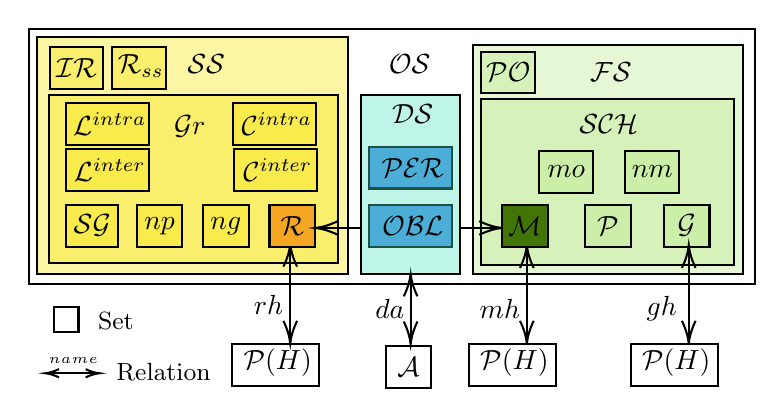
\begin{tikzpicture}[x=0.75pt,y=0.75pt,yscale=-1,xscale=1]
%uncomment if require: \path (0,1800); %set diagram left start at 0, and has height of 1800

%Shape: Rectangle [id:dp9341453924522656] 
\draw  [fill={rgb, 255:red, 255; green, 255; blue, 255 }  ,fill opacity=1 ] (160,44) -- (510,44) -- (510,167) -- (160,167) -- cycle ;
%Shape: Rectangle [id:dp4628140741854456] 
\draw  [fill={rgb, 255:red, 184; green, 233; blue, 134 }  ,fill opacity=0.34 ] (374,52) -- (504,52) -- (504,162) -- (374,162) -- cycle ;
%Shape: Rectangle [id:dp6461749357206974] 
\draw  [fill={rgb, 255:red, 184; green, 233; blue, 134 }  ,fill opacity=0.34 ] (378,78) -- (500,78) -- (500,158) -- (378,158) -- cycle ;
%Shape: Rectangle [id:dp47018118728898073] 
\draw  [fill={rgb, 255:red, 248; green, 231; blue, 28 }  ,fill opacity=0.4 ] (164,48) -- (314,48) -- (314,162) -- (164,162) -- cycle ;
%Straight Lines [id:da37904402438854] 
\draw    (400,150.31) -- (400,193.69) ;
\draw [shift={(400,195.69)}, rotate = 270] [color={rgb, 255:red, 0; green, 0; blue, 0 }  ][line width=0.75]    (10.93,-3.29) .. controls (6.95,-1.4) and (3.31,-0.3) .. (0,0) .. controls (3.31,0.3) and (6.95,1.4) .. (10.93,3.29)   ;
\draw [shift={(400,148.31)}, rotate = 90] [color={rgb, 255:red, 0; green, 0; blue, 0 }  ][line width=0.75]    (10.93,-3.29) .. controls (6.95,-1.4) and (3.31,-0.3) .. (0,0) .. controls (3.31,0.3) and (6.95,1.4) .. (10.93,3.29)   ;
%Straight Lines [id:da30557994145553513] 
\draw    (368,140) -- (386,140) ;
\draw [shift={(388,140)}, rotate = 180] [color={rgb, 255:red, 0; green, 0; blue, 0 }  ][line width=0.75]    (10.93,-3.29) .. controls (6.95,-1.4) and (3.31,-0.3) .. (0,0) .. controls (3.31,0.3) and (6.95,1.4) .. (10.93,3.29)   ;
%Shape: Rectangle [id:dp15689957472567295] 
\draw  [fill={rgb, 255:red, 248; green, 231; blue, 28 }  ,fill opacity=0.4 ] (169.56,76) -- (309.06,76) -- (309.06,157) -- (169.56,157) -- cycle ;
%Shape: Rectangle [id:dp6202366628126772] 
\draw  [fill={rgb, 255:red, 255; green, 255; blue, 255 }  ,fill opacity=1 ] (372,196) -- (414,196) -- (414,216) -- (372,216) -- cycle ;

%Shape: Rectangle [id:dp20067598884831228] 
\draw  [fill={rgb, 255:red, 248; green, 231; blue, 28 }  ,fill opacity=0.4 ] (212.06,129) -- (234.06,129) -- (234.06,149) -- (212.06,149) -- cycle ;

%Shape: Rectangle [id:dp5970765798398485] 
\draw  [fill={rgb, 255:red, 248; green, 231; blue, 28 }  ,fill opacity=0.4 ] (178.06,129) -- (203.06,129) -- (203.06,149) -- (178.06,149) -- cycle ;
%Shape: Rectangle [id:dp92237875722883] 
\draw  [fill={rgb, 255:red, 248; green, 231; blue, 28 }  ,fill opacity=0.4 ] (178.06,102) -- (218.06,102) -- (218.06,122) -- (178.06,122) -- cycle ;

%Shape: Rectangle [id:dp6591761395302378] 
\draw  [fill={rgb, 255:red, 248; green, 231; blue, 28 }  ,fill opacity=0.4 ] (178.06,80) -- (218.06,80) -- (218.06,100) -- (178.06,100) -- cycle ;

%Shape: Rectangle [id:dp11794703752595392] 
\draw  [fill={rgb, 255:red, 248; green, 231; blue, 28 }  ,fill opacity=0.4 ] (258.5,80) -- (298.5,80) -- (298.5,100) -- (258.5,100) -- cycle ;

%Shape: Rectangle [id:dp6557958558103134] 
\draw  [fill={rgb, 255:red, 248; green, 231; blue, 28 }  ,fill opacity=0.4 ] (259,102) -- (299,102) -- (299,122) -- (259,122) -- cycle ;

%Shape: Rectangle [id:dp8284992701408749] 
\draw  [fill={rgb, 255:red, 65; green, 117; blue, 5 }  ,fill opacity=1 ] (388,129) -- (410,129) -- (410,149) -- (388,149) -- cycle ;

%Shape: Rectangle [id:dp7066110016250453] 
\draw  [fill={rgb, 255:red, 248; green, 231; blue, 28 }  ,fill opacity=0.4 ] (244,129) -- (266,129) -- (266,149) -- (244,149) -- cycle ;

%Shape: Rectangle [id:dp4021333114319714] 
\draw  [fill={rgb, 255:red, 248; green, 231; blue, 28 }  ,fill opacity=0.4 ] (170.31,53) -- (195.69,53) -- (195.69,73) -- (170.31,73) -- cycle ;

%Shape: Rectangle [id:dp8476756388266236] 
\draw  [fill={rgb, 255:red, 248; green, 231; blue, 28 }  ,fill opacity=0.4 ] (200,53) -- (226,53) -- (226,73) -- (200,73) -- cycle ;

%Shape: Rectangle [id:dp07470576340681823] 
\draw  [fill={rgb, 255:red, 74; green, 144; blue, 226 }  ,fill opacity=1 ] (324,101) -- (364,101) -- (364,121) -- (324,121) -- cycle ;

%Shape: Rectangle [id:dp31407652093057714] 
\draw  [fill={rgb, 255:red, 74; green, 144; blue, 226 }  ,fill opacity=1 ] (324,129) -- (364,129) -- (364,149) -- (324,149) -- cycle ;

%Shape: Rectangle [id:dp053729126169398844] 
\draw  [fill={rgb, 255:red, 184; green, 233; blue, 134 }  ,fill opacity=0.34 ] (378,55) -- (404,55) -- (404,75) -- (378,75) -- cycle ;

%Shape: Rectangle [id:dp7720103442630182] 
\draw  [fill={rgb, 255:red, 184; green, 233; blue, 134 }  ,fill opacity=0.34 ] (405.94,103) -- (431.94,103) -- (431.94,123) -- (405.94,123) -- cycle ;

%Shape: Rectangle [id:dp3183552657000306] 
\draw  [fill={rgb, 255:red, 184; green, 233; blue, 134 }  ,fill opacity=0.34 ] (447.44,103) -- (473.44,103) -- (473.44,123) -- (447.44,123) -- cycle ;

%Shape: Rectangle [id:dp10802424702469593] 
\draw  [fill={rgb, 255:red, 184; green, 233; blue, 134 }  ,fill opacity=0.34 ] (466,129) -- (488,129) -- (488,149) -- (466,149) -- cycle ;

%Shape: Rectangle [id:dp16589412198505937] 
\draw  [fill={rgb, 255:red, 184; green, 233; blue, 134 }  ,fill opacity=0.34 ] (428,129) -- (450,129) -- (450,149) -- (428,149) -- cycle ;

%Shape: Rectangle [id:dp1270989692188249] 
\draw  [fill={rgb, 255:red, 255; green, 255; blue, 255 }  ,fill opacity=1 ] (258,196) -- (300,196) -- (300,216) -- (258,216) -- cycle ;

%Straight Lines [id:da40017392935840324] 
\draw    (286,149.69) -- (286,193.69) ;
\draw [shift={(286,195.69)}, rotate = 270] [color={rgb, 255:red, 0; green, 0; blue, 0 }  ][line width=0.75]    (10.93,-3.29) .. controls (6.95,-1.4) and (3.31,-0.3) .. (0,0) .. controls (3.31,0.3) and (6.95,1.4) .. (10.93,3.29)   ;
\draw [shift={(286,147.69)}, rotate = 90] [color={rgb, 255:red, 0; green, 0; blue, 0 }  ][line width=0.75]    (10.93,-3.29) .. controls (6.95,-1.4) and (3.31,-0.3) .. (0,0) .. controls (3.31,0.3) and (6.95,1.4) .. (10.93,3.29)   ;
%Shape: Rectangle [id:dp21027747628033966] 
\draw  [fill={rgb, 255:red, 245; green, 166; blue, 35 }  ,fill opacity=1 ] (276,129) -- (298,129) -- (298,149) -- (276,149) -- cycle ;

%Shape: Rectangle [id:dp5582162899072272] 
\draw  [fill={rgb, 255:red, 255; green, 255; blue, 255 }  ,fill opacity=1 ] (172,178) -- (184,178) -- (184,190) -- (172,190) -- cycle ;
%Straight Lines [id:da3472969066473863] 
\draw    (170,210) -- (192,210) ;
\draw [shift={(194,210)}, rotate = 180] [color={rgb, 255:red, 0; green, 0; blue, 0 }  ][line width=0.75]    (6.56,-1.97) .. controls (4.17,-0.84) and (1.99,-0.18) .. (0,0) .. controls (1.99,0.18) and (4.17,0.84) .. (6.56,1.97)   ;
\draw [shift={(168,210)}, rotate = 0] [color={rgb, 255:red, 0; green, 0; blue, 0 }  ][line width=0.75]    (6.56,-1.97) .. controls (4.17,-0.84) and (1.99,-0.18) .. (0,0) .. controls (1.99,0.18) and (4.17,0.84) .. (6.56,1.97)   ;
%Shape: Rectangle [id:dp07012270906311535] 
\draw  [fill={rgb, 255:red, 255; green, 255; blue, 255 }  ,fill opacity=1 ] (332,197) -- (354,197) -- (354,217) -- (332,217) -- cycle ;

%Straight Lines [id:da7534392810513293] 
\draw    (344,164) -- (344,194) ;
\draw [shift={(344,196)}, rotate = 270] [color={rgb, 255:red, 0; green, 0; blue, 0 }  ][line width=0.75]    (10.93,-3.29) .. controls (6.95,-1.4) and (3.31,-0.3) .. (0,0) .. controls (3.31,0.3) and (6.95,1.4) .. (10.93,3.29)   ;
\draw [shift={(344,162)}, rotate = 90] [color={rgb, 255:red, 0; green, 0; blue, 0 }  ][line width=0.75]    (10.93,-3.29) .. controls (6.95,-1.4) and (3.31,-0.3) .. (0,0) .. controls (3.31,0.3) and (6.95,1.4) .. (10.93,3.29)   ;
%Straight Lines [id:da4125176624573814] 
\draw    (320,140) -- (300,140) ;
\draw [shift={(298,140)}, rotate = 360] [color={rgb, 255:red, 0; green, 0; blue, 0 }  ][line width=0.75]    (10.93,-3.29) .. controls (6.95,-1.4) and (3.31,-0.3) .. (0,0) .. controls (3.31,0.3) and (6.95,1.4) .. (10.93,3.29)   ;
%Shape: Rectangle [id:dp005426842763594397] 
\draw  [fill={rgb, 255:red, 80; green, 227; blue, 194 }  ,fill opacity=0.36 ] (320,76) -- (368,76) -- (368,162) -- (320,162) -- cycle ;
%Straight Lines [id:da9128713017721406] 
\draw    (478,150.31) -- (478,193.69) ;
\draw [shift={(478,195.69)}, rotate = 270] [color={rgb, 255:red, 0; green, 0; blue, 0 }  ][line width=0.75]    (10.93,-3.29) .. controls (6.95,-1.4) and (3.31,-0.3) .. (0,0) .. controls (3.31,0.3) and (6.95,1.4) .. (10.93,3.29)   ;
\draw [shift={(478,148.31)}, rotate = 90] [color={rgb, 255:red, 0; green, 0; blue, 0 }  ][line width=0.75]    (10.93,-3.29) .. controls (6.95,-1.4) and (3.31,-0.3) .. (0,0) .. controls (3.31,0.3) and (6.95,1.4) .. (10.93,3.29)   ;
%Shape: Rectangle [id:dp7604827971406838] 
\draw  [fill={rgb, 255:red, 255; green, 255; blue, 255 }  ,fill opacity=1 ] (450,196) -- (492,196) -- (492,216) -- (450,216) -- cycle ;



% Text Node
\draw (465,179) node   [align=left] {$gh$};
% Text Node
\draw (181.5,204) node  [font=\tiny] [align=left] {$name$};
% Text Node
\draw (334,179) node   [align=left] {$da$};
% Text Node
\draw (222,207) node  [font=\footnotesize] [align=left] {\begin{minipage}[lt]{29.67pt}\setlength\topsep{0pt}
\begin{center}
{\small Relation}
\end{center}

\end{minipage}};
% Text Node
\draw (202,185) node  [font=\footnotesize] [align=left] {\begin{minipage}[lt]{13.75pt}\setlength\topsep{0pt}
\begin{center}
{\small Set}
\end{center}

\end{minipage}};
% Text Node
\draw (343.5,61) node   [align=left] {$\mathcal{OS}$};
% Text Node
\draw (190.56,139) node   [align=left] {$\mathcal{SG}$};
% Text Node
\draw (345,85) node   [align=left] {$\mathcal{DS}$};
% Text Node
\draw (245.5,61) node   [align=left] {$\mathcal{SS}$};
% Text Node
\draw (387,179) node   [align=left] {$mh$};
% Text Node
\draw (275.5,177) node   [align=left] {$rh$};
% Text Node
\draw (237.56,91) node   [align=left] {$\mathcal{G}r$};
% Text Node
\draw (440.5,65) node   [align=left] {$\mathcal{FS}$};
% Text Node
\draw (439.44,90) node   [align=left] {$\mathcal{SCH}$};
% Text Node
\draw (472,205) node   [align=left] {$\mathcal{P}(H)$};
% Text Node
\draw (343,207) node   [align=left] {$\mathcal{A}$};
% Text Node
\draw (287,139) node   [align=left] {$\mathcal{R}$};
% Text Node
\draw (280,205) node   [align=left] {$\mathcal{P}(H)$};
% Text Node
\draw (439,139) node   [align=left] {$\mathcal{P}$};
% Text Node
\draw (477,139) node   [align=left] {$\mathcal{G}$};
% Text Node
\draw (460.44,113) node   [align=left] {$nm$};
% Text Node
\draw (418.94,113) node   [align=left] {$mo$};
% Text Node
\draw (391,65) node   [align=left] {$\mathcal{PO}$};
% Text Node
\draw (345,139) node   [align=left] {$\mathcal{OBL}$};
% Text Node
\draw (345,111) node   [align=left] {$\mathcal{PER}$};
% Text Node
\draw (214,62) node   [align=left] {$\mathcal{R}_{ss}$};
% Text Node
\draw (183,63) node   [align=left] {$\mathcal{IR}$};
% Text Node
\draw (255,139) node   [align=left] {$\mathnormal{ng}$};
% Text Node
\draw (399,139) node   [align=left] {$\mathcal{M}$};
% Text Node
\draw (280,112) node   [align=left] {$\mathcal{C}^{inter}$};
% Text Node
\draw (279.5,90) node   [align=left] {$\mathcal{C}^{intra}$};
% Text Node
\draw (199.06,90) node   [align=left] {$\mathcal{L}^{intra}$};
% Text Node
\draw (199.06,112) node   [align=left] {$\mathcal{L}^{inter}$};
% Text Node
\draw (223.06,139) node   [align=left] {$np$};
% Text Node
\draw (394,205) node   [align=left] {$\mathcal{P}(H)$};


\end{tikzpicture}
    \caption{Relations entre les spécifications organisationnelles et les sous-ensembles historiques}
    \label{fig:PRAHOM_osm_rels}
\end{figure}

Un sous-ensemble historique contraint une politique à un rôle. Nous introduisons des \textbf{contraintes de politique observables} $c\pi: H \times \Omega \rightarrow \mathcal{P}(A)$, qui dictent les actions autorisées par observation. Ces contraintes s'intègrent dans les politiques selon trois modes :
\begin{itemize}
    \item \textbf{Correct} : ajuste toute action choisie $\pi(\omega)$ à une action attendue dans $c\pi(\omega)$, garantissant ainsi la sécurité.
    \item \textbf{Pénaliser} : ajoute une pénalité pour les actions $\pi(\omega) \notin c\pi(\omega)$, encourageant les agents à apprendre les contraintes.
    \item \textbf{Correct\_Policy} : crée une \textbf{politique contrainte} $\pi_c$ où $c\pi$ corrige $\pi$, garantissant la sécurité interne.
\end{itemize}

\subsection{Spécifications fonctionnelles}

\textbf{Spécifications fonctionnelles} ($\mathcal{FS} = \langle \mathcal{SCH}, \mathcal{PO} \rangle$) définissent les tâches et les objectifs :
\begin{itemize}
    \item $\mathcal{SCH} = \langle \mathcal{G}, \mathcal{M}, \mathcal{P}, mo, nm \rangle$ : schémas sociaux, où :
          \begin{itemize}
              \item $\mathcal{G}$ : objectifs globaux.
              \item $\mathcal{M}$ : Étiquettes de mission.
              \item $\mathcal{P}$ : Plans $(g_f, \{g_i\}_{0 \leq i \leq s}, op, ps)$.
              \item $mo$ : objectifs pour chaque mission.
              \item $nm$ : Cardinalité des agents par mission.
          \end{itemize}
    \item $\mathcal{PO}$ : Ordres de préférence $(m_1 \prec m_2)$.
\end{itemize}

Les objectifs sont représentés sous forme de sous-ensembles d'historique, $gh: \mathcal{G} \rightarrow \mathcal{P}(H)$. Les missions sont mappées à des historiques attendus $mh: \mathcal{M} \rightarrow \mathcal{P}(H)$. Les objectifs ont un impact sur le MARL en mettant à jour la fonction de récompense, incitant les agents à générer les historiques souhaités. Nous introduisons des \textbf{fonctions de récompense observables} $R_g: H \rightarrow \mathbb{R}$, qui mesurent la proximité des histoires générées par rapport à celles attendues. Les récompenses des missions sont des sommes pondérées des récompenses des objectifs, ce qui favorise une convergence plus rapide.

\subsection{Spécifications déontiques}

\textbf{Spécifications déontiques} ($\mathcal{DS} = \langle \mathcal{OBL}, \mathcal{PER} \rangle$) définissent les permissions et les obligations :
\begin{itemize}
    \item $\mathcal{TC}$ : Contraintes temporelles.
    \item $\mathcal{OBL}$ : Obligations $(obl(\rho_a, m, tc))$.
    \item $\mathcal{PER}$ : autorisations $(per(\rho_a, m, tc))$.
\end{itemize}

La relation $da: \mathcal{PER} \cup \mathcal{OBL} \rightarrow \mathcal{P}(\mathcal{A})$ contraint les rôles et les missions avec des limites de temps, gérées par $dttl: \mathcal{PER} \cup \mathcal{OBL} \times \mathcal{A} \rightarrow \mathbb{N}$. Les obligations ont des multiplicateurs de récompense plus élevés que les autorisations, ce qui donne la priorité au respect des missions.

Ces principes intègrent les spécifications organisationnelles dans le cadre MARL, formant ainsi l'algorithme CoPRAHOM.

\section{Un algorithme MARL orienté cyberdéfense}\label{sec:coprahom}

Dans cette section, nous récapitulons brièvement l'architecture MASCARA en tant que modèle organisationnel abstrait général de cyberdéfense $\mathcal{M}OISE^+$ à utiliser conjointement avec CoPRAHOM.
Nous détaillons ensuite l'algorithme CoPRAHOM ainsi que sa mise en œuvre pratique dans des scénarios concrets de cyberdéfense.
%Nous présentons CoPRAHOM, un nouvel algorithme qui intègre l'architecture MASCARA aux principes de $\mathcal{M}OISE^+$ afin de relever les défis de la cyberdéfense dans le cadre de l'apprentissage par renforcement multi-agents (MARL). Cette intégration facilite la formation d'agents qui adhèrent à des rôles et missions organisationnels prédéfinis dans le contexte de la cyberdéfense.

\subsection{Une architecture générale de cyberdéfense comme fondement}

L'architecture MASCARA est conçue pour les AICA. Elle comprend des composants tels qu'un moteur de prise de décision, une base de connaissances, un moteur d'apprentissage en ligne, un moteur de comportement des agents, un orchestrateur, un espace de travail, une interface de collaboration et un protocole de communication interne. Ces composants fonctionnent ensemble pour surveiller, détecter et répondre aux cybermenaces.
%
% La conversion de l'architecture MASCARA en modèle $\mathcal{M}OISE^+$ présente des avantages pour relever divers défis en matière de cyberdéfense, car :

% \begin{itemize}
%     \item \textbf{Représentation structurée} : $\mathcal{M}OISE^+$ fournit une représentation structurée des rôles, des interactions et des objectifs, qui s'aligne bien avec la nature hiérarchique et fonctionnelle de MASCARA.
%     \item \textbf{Spécification des rôles et des missions} : $\mathcal{M}OISE^+$ permet une spécification précise des rôles et des missions, garantissant que le comportement de chaque agent est aligné sur la stratégie globale de cyberdéfense.
%     \item \textbf{Relations déontiques} : La spécification déontique dans $\mathcal{M}OISE^+$ aide à définir les autorisations et les obligations des agents, ce qui est crucial dans un environnement de cyberdéfense dynamique et réactif.
% \end{itemize}

Le modèle organisationnel général abstrait de cyberdéfense dérivé de MASCARA peut être représenté à l'aide de $\mathcal{M}OISE^+$. Les plus importants sont les suivants :
%
% \begin{itemize}
%     \item \textbf{Spécifications structurelles} ($\mathcal{SS}$) : définir des rôles tels que \textit{Détecteur d'intrusion}, \textit{Analyseur de trafic}, \textit{Coordinateur de réponse} et leurs relations.
%     \item \textbf{Spécifications fonctionnelles} ($\mathcal{FS}$) : définir des missions telles que \textit{Détecter les intrusions}, \textit{Analyser le trafic malveillant} et \textit{Atténuer les attaques}, chacune avec des objectifs et des plans spécifiques.
%     \item \textbf{Spécifications déontiques} ($\mathcal{DS}$) : Définir les autorisations et les obligations des rôles pour s'engager dans des missions en fonction de la connaissance de la situation et de règles prédéfinies.
% \end{itemize}
%
% Pour relier chaque rôle ou mission à un sous-ensemble d'historique attendu, il est nécessaire de définir des modèles, des protocoles, une logique et des règles que les agents doivent respecter. Ci-dessous, nous présentons un cadre permettant de relier les rôles aux sous-ensembles d'historique attendus :
%
\textbf{Détecteur d'intrusion} qui implique la surveillance continue du trafic réseau, la génération d'alertes en cas de détection d'anomalies et l'utilisation de modèles statistiques et d'algorithmes de détection d'anomalies.
%
\textbf{Analyseur de trafic} qui se concentre sur l'analyse du contenu des paquets à la recherche de signatures malveillantes, la corrélation des données provenant de plusieurs sources et l'utilisation de techniques d'inspection approfondie des paquets et de correspondance des signatures.
%
\textbf{Coordinateur de réponse} qui exécute des plans de réponse prédéfinis, coordonne les autres agents pour une réponse synchronisée et évalue l'impact des différentes stratégies de réponse.


Les missions les plus pertinentes comprennent :
%
\textbf{Détection des intrusions}, qui vise à identifier les tentatives d'accès non autorisés, à déployer des honeypots pour attirer les attaquants et à mettre à jour les règles de détection en fonction des menaces émergentes.
%
\textbf{Analyser le trafic malveillant} qui vise à collecter et examiner les données de trafic ; utiliser des modèles d'apprentissage automatique pour classer le trafic ; et corréler les résultats avec des modèles d'attaque connus.
%
\textbf{Atténuer les attaques} qui vise à déployer des contre-mesures contre les menaces identifiées ; isoler les systèmes affectés et rediriger le trafic ; et hiérarchiser les mesures qui minimisent les interruptions de service.

Cette présentation générale présente un modèle abstrait appelé \textit{MASCARA-$\mathcal{M}OISE^+$}, conçu comme un cadre flexible permettant de spécifier des rôles, des missions et des interactions personnalisés dans divers scénarios. Le concept central de CoPRAHOM exploite la capacité à définir partiellement les rôles ou les missions du modèle susmentionné à travers leurs sous-ensembles d'historique attendus associés. Cette définition partielle permet un ajustement adaptatif à mesure que surviennent des situations nouvelles ou imprévues qui n'étaient pas couvertes à l'origine. Cette prémisse a donc conduit à l'algorithme CoPRAHOM pour la mise en œuvre de mécanismes visant à guider et à contraindre les agents, les obligeant à respecter ces rôles et missions prédéfinis. Cette approche facilite non seulement la surveillance en temps réel des activités des agents, mais garantit également que leurs comportements restent conformes aux exigences.


\subsection{CoPRAHOM pour les scénarios de cyberdéfense}

L'algorithme CoPRAHOM nécessite tout d'abord de définir un modèle organisationnel concret $\mathcal{M}OISE^+$ (à partir du modèle \textit{MASCARA-$\mathcal{M}OISE^+$}) et de décrire comment chaque rôle ou mission doit se présenter en termes de sous-ensembles historiques dans MARL.
% Il permet ensuite d'intégrer systématiquement les spécifications organisationnelles dans le processus d'apprentissage en imposant des contraintes sur les politiques conjointes basées sur des rôles, des missions et des relations d'autorisation/obligation prédéfinis.
Cette intégration garantit que les comportements des agents sont non seulement optimisés en termes de performances, mais également conformes aux exigences organisationnelles.
%
Dans cette section, nous présentons de manière informelle une description détaillée, étape par étape, de l'algorithme CoPRAHOM et discutons de sa mise en œuvre dans le \textit{CoPRAHOM Wrapper}.\\

\textbf{Initialisation et paramètres d'entrée} :
Tout d'abord, CoPRAHOM initialise la politique conjointe avec la politique conjointe initiale et règle le compteur d'épisodes sur zéro. Il définit également une variable booléenne appelée « sufficient » sur False, indiquant que la récompense cumulée attendue n'a pas encore été atteinte. Elle est initialisée avec le rôle par rapport à l'historique $rh$, la mission par rapport à l'historique $mh$ et les spécifications déontiques de l'agent $da$ qui décrivent comment les agents doivent être influencés pendant l'apprentissage par des rôles et des missions prédéfinis.

\textbf{Étape 1 : Déterminer les contraintes de politique observable conjointe} :
Identifier les contraintes de politique observables conjointes à partir des spécifications organisationnelles à l'aide des relations $rh$ et $da$.

\textbf{Étape 2 : Initialiser la politique contrainte} :
Si le mode d'intégration des contraintes est défini sur « corriger la politique », créez et utilisez une politique conjointe contrainte basée sur la politique initiale et les contraintes de politique observables.

\textbf{Étape 3 : Déterminer les fonctions de récompense observables} :
Établissez les fonctions de récompense observables à partir des spécifications organisationnelles. Intégrez ces fonctions de récompense observables dans la fonction de récompense globale.

\textbf{Étape 4 : Boucle d'entraînement principale} :
Exécutez la boucle d'entraînement principale pendant un nombre maximal d'épisodes ou jusqu'à ce que l'espérance de récompense cumulative soit atteinte.

\textbf{Initialiser l'épisode} :
Au début de chaque épisode, réinitialisez l'environnement, les observations et l'historique des actions. Réinitialisez la récompense et la pénalité cumulées. Initialisez les valeurs de durée de vie des autorisations/obligations et définissez l'observation et l'action initiales par l'environnement.

\textbf{Parcourir l'épisode} :
Au cours de chaque épisode, effectuez les étapes suivantes pour un nombre maximal d'étapes :

\begin{itemize}
    \item Mettre à jour la politique conjointe à l'aide de l'algorithme MARL en fonction de l'historique actuel et des dernières récompenses ;
    \item Sélectionnez l'action suivante en fonction de l'observation actuelle ;
    \item Identifier les actions attendues à partir des contraintes observables de la politique. Si l'action sélectionnée ne figure pas parmi les actions attendues, la corriger ou la pénaliser en fonction du mode d'intégration des contraintes ;
    \item Mettre à jour l'historique actuel et appliquer l'action à l'environnement pour obtenir la prochaine observation et récompense, en ajoutant les pénalités encourues ;
    \item Diminuer les valeurs de durée de vie et mettre à jour les fonctions de récompense et les politiques si certaines spécifications organisationnelles ont changé.
\end{itemize}

\textbf{Vérification de la suffisance} :
Après chaque épisode, vérifiez si la récompense cumulative correspond à l'espérance et incrémentez le compteur d'épisodes.


% \quad \emph{Implémentation} :
% Le wrapper utilise la fonction \textit{train\_under\_constraint()} proposée pour gérer ces initialisations, en acceptant les paramètres d'entrée et en définissant le compteur d'épisodes et la condition de suffisance. Cette fonction prend au moins deux arguments : les objets \textit{ol\_mngr} et \textit{os} :

% Le singleton \textit{ol\_mngr} fait partie de l'API. Il utilise le modèle de transformateur HuggingFace \textit{tiiuae/falcon-7b} pour apprendre les correspondances entre les observations réelles et les étiquettes courtes, en conjonction avec un dictionnaire simple. Il fournit également un processus interactif permettant aux utilisateurs d'étiqueter chaque observation pendant la procédure d'étiquetage, ce qui est essentiel pour détecter et catégoriser avec précision les cybermenaces dans un environnement dynamique. Son intérêt réside dans son utilisation au sein d'un \textit{history\_subset}. Cette classe gère les sous-ensembles d'historique en fonction de modèles ou de règles prédéfinis via un graphe d'historique implémenté lors du traitement des modèles. \textit{ol\_mngr} facilite la création d'un modèle en permettant aux utilisateurs d'utiliser des étiquettes explicites pour créer facilement un comportement attendu. Il est également possible d'utiliser des fonctions personnalisées au sein d'un history\_subset, ce qui offre une grande flexibilité pour s'adapter à divers scénarios de cyberdéfense.

% La classe \textit{osr} représente un modèle organisationnel $\mathcal{M}OISE^+$ dans une représentation de type JSON et constitue l'épine dorsale du \emph{CoPRAHOM Wrapper}. Dans cette classe, les rôles et les objectifs sont directement mappés à des contraintes de politique observables \textit{opc} et à des fonctions de récompense observables \textit{orf} à l'aide de modèles, de règles ou de fonctions personnalisées. Cette classe implémente les mappages rôle-historique (rh), objectif-historique (gh) et mission-historique (mh). Les autorisations et les obligations sont également définies ici, chaque obligation ou autorisation étant mappée à des agents, implémentant ainsi la relation spécification déontique-agents (da).

\

Pour implémenter CoPRAHOM, nous avons privilégié la bibliothèque \emph{PettingZoo}, qui offre une API largement utilisée et standardisée pour développer des environnements multi-agents et utiliser des algorithmes MARL~\cite{terry2020pettingzoo}. Nous avons intégré la bibliothèque MARLlib~\cite{hu2022marllib}, qui offre un nombre important d'algorithmes MARL implémentés, tels que MAPPO ou MADDPG, ainsi que des modèles affinés pour un large éventail d'environnements. Cette implémentation a donné naissance au \textit{CoPRAHOM Wrapper}, qui étend l'API PettingZoo avec des fonctionnalités supplémentaires spécifiques à CoPRAHOM.
%
Le CoPRAHOM Wrapper fournit une API avec des classes auxiliaires supplémentaires pour définir les spécifications organisationnelles et les relier à leur comportement attendu dans un contexte de cyberdéfense. Ces deux classes principales sont les objets \textit{ol\_mngr} et \textit{osr}.

La classe singleton \textit{ol\_mngr}, qui fait partie de l'API, utilise le modèle de transformateur HuggingFace \textit{tiiuae/falcon-7b} pour apprendre les mappages en conjonction avec un dictionnaire simple.
%Elle fournit également un processus interactif permettant aux utilisateurs d'étiqueter chaque observation pendant la procédure d'étiquetage, ce qui est essentiel pour détecter et catégoriser avec précision les cybermenaces dans un environnement dynamique.
La classe \textit{osr} rassemble tous les éléments précédemment instanciés dans un modèle organisationnel $\mathcal{M}OISE^+$ complet, qui peut être représenté au format JSON. Dans cette classe, les rôles et les objectifs sont directement mappés à des objets \textit{opc} de contrainte de politique observable et \textit{orf} de fonction de récompense observable à l'aide de modèles, de règles ou de fonctions personnalisées. Cette classe implémente les mappages rôle-historique (rh), objectif-historique (gh) et mission-historique (mh). Les autorisations et les obligations sont également définies ici, chaque obligation ou autorisation étant mappée à des agents, ce qui implémente la relation d'allocation déontique (da).

Une fois que l'environnement PettingZoo est encapsulé dans le wrapper CoPRAHOM et que toutes les classes auxiliaires ont été instanciées pour obtenir un \textit{ol\_mngr} et un \textit{os}, l'API du wrapper fournit la fonction \textit{train\_under\_constraint()}. Cette fonction permet d'exécuter l'algorithme CoPRAHOM, en prenant comme arguments les objets \textit{ol\_mngr} et \textit{os}, en plus d'autres paramètres MARLlib. Au final, elle génère des objets de politique MARLlib et des données statistiques, garantissant que les agents sont formés pour répondre aux exigences strictes des opérations de cyberdéfense.

\section{Configuration expérimentale}\label{sec:experimental_setup}

Afin de répondre aux exigences du 3e défi CAGE, notre configuration expérimentale consiste à créer des modèles MAS de cyberdéfense à l'aide des spécifications organisationnelles $\mathcal{M}OISE^+$. Nous avons établi des modèles avec différents niveaux de contraintes, notamment différents rôles et missions. Pour nous inspirer, nous nous sommes référés à l'architecture MASCARA lors du développement de ces modèles. Après avoir mis en œuvre CoPRAHOM, nous avons démontré son utilisation dans l'intégration des modèles définis afin de contraindre l'apprentissage des agents. Enfin, nous avons évalué l'impact de ces modèles pendant la formation et après le déploiement.

\subsection{3e défi CAGE}

Comme illustré dans \autoref{fig:cage_challenge},
Le 3e défi CAGE simule un conflit frontalier fictif dans lequel Florin utilise des drones autonomes pour ses communications militaires. Le simulateur CybORG modélise un essaim de drones formant un réseau ad hoc, qui doit être défendu contre des programmes malveillants (agents rouges) implantés par les espions de Guilder. L'objectif est de créer des systèmes de défense autonomes (agents bleus) qui détectent, répondent et atténuent les attaques, assurant ainsi une communication continue pour les troupes de Florin (agents verts).

\begin{figure}
    \centering
    \begin{tikzpicture}
    % Define the positions of the drones
    \coordinate (A) at (0,2);
    \coordinate (B) at (2,2);
    \coordinate (C) at (1,3);
    \coordinate (D) at (3,3);
    \coordinate (E) at (4,2);
    \coordinate (F) at (5,3);
    \coordinate (G) at (6,2);
    
    % Draw the drones with the drone image
    \foreach \pos in {A,B,C,D,E,F,G} {
        \node at (\pos) {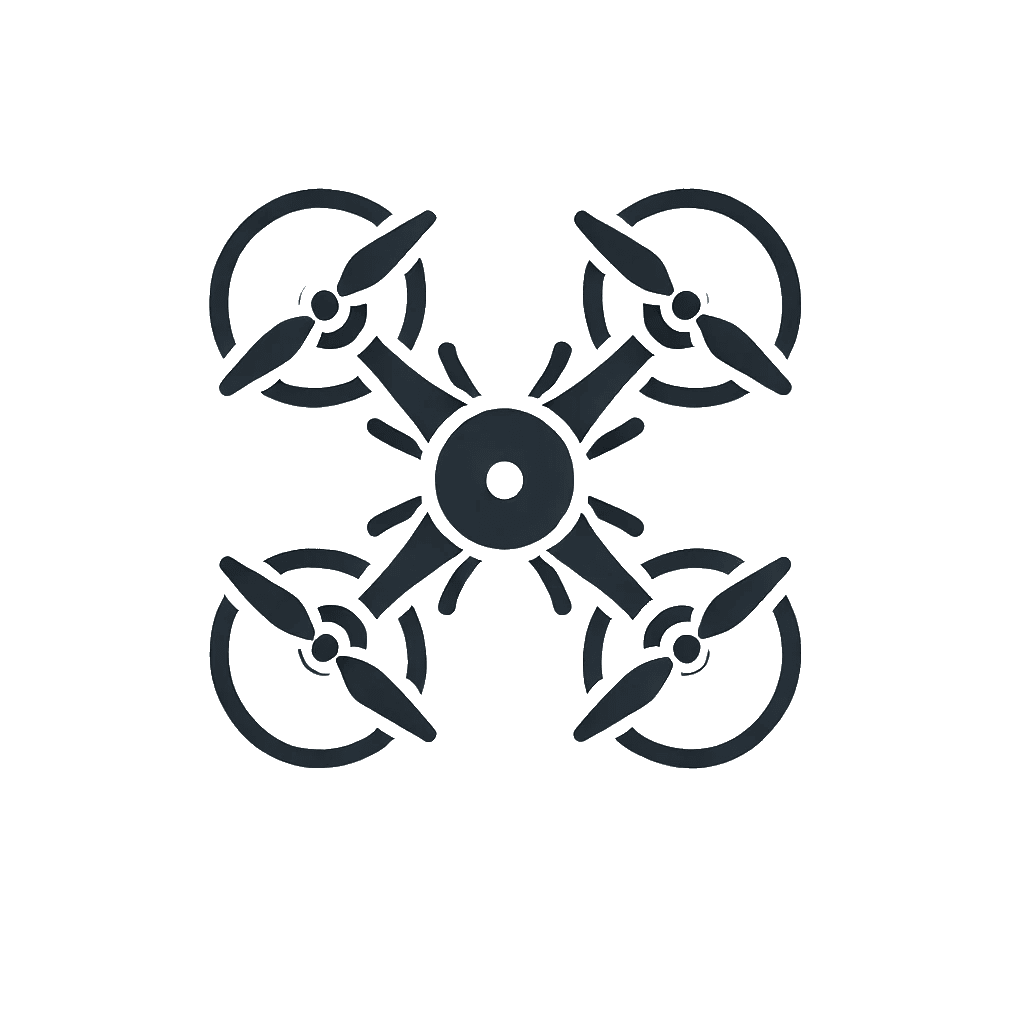
\includegraphics[width=1cm]{figures/drone_scheme.png}};
    }
    
    % Draw the connections
    \draw[dotted] (A) -- (B);
    \draw[dotted] (B) -- (C);
    % \draw[dotted] (B) -- (D);
    \draw[dotted] (D) -- (E);
    \draw[dotted] (E) -- (F);
    % \draw[dotted] (F) -- (G);
    
    % Add agent symbols as green circles
    \node[fill=green, circle, minimum size=7pt, inner sep=0pt] at (0.41,2.41) {};
    \node[fill=green, circle, minimum size=7pt, inner sep=0pt] at (2.41,2.41) {};
    \node[fill=green, circle, minimum size=7pt, inner sep=0pt] at (1.41,3.41) {};
    \node[fill=green, circle, minimum size=7pt, inner sep=0pt] at (3.41,3.41) {};
    \node[fill=green, circle, minimum size=7pt, inner sep=0pt] at (4.41,2.41) {};
    \node[fill=green, circle, minimum size=7pt, inner sep=0pt] at (5.41,3.41) {};
    \node[fill=green, circle, minimum size=7pt, inner sep=0pt] at (6.41,2.41) {};
    
    % Add blue circles to the left of some green circles
    \node[fill=blue, circle, minimum size=7pt, inner sep=0pt] at (0.11,2.41) {};
    \node[fill=blue, circle, minimum size=7pt, inner sep=0pt] at (2.11,2.41) {};
    \node[fill=blue, circle, minimum size=7pt, inner sep=0pt] at (3.11,3.41) {};
    \node[fill=blue, circle, minimum size=7pt, inner sep=0pt] at (5.11,3.41) {};
    
    % Add one additional circle to the left of an existing circle
    \node[fill=red, circle, minimum size=7pt, inner sep=0pt] at (4.11,2.41) {}; % Example: red circle added

    % Add the legend
    \node[fill=red, circle, minimum size=7pt, inner sep=0pt, label=right:{\small red agent}] at (0,1) {};
    \node[fill=blue, circle, minimum size=7pt, inner sep=0pt, label=right:{\small blue agent}] at (3,1) {};
    \node[fill=green, circle, minimum size=7pt, inner sep=0pt, label=right:{\small green agent}] at (6,1) {};
    
    \node at (1,0.5) {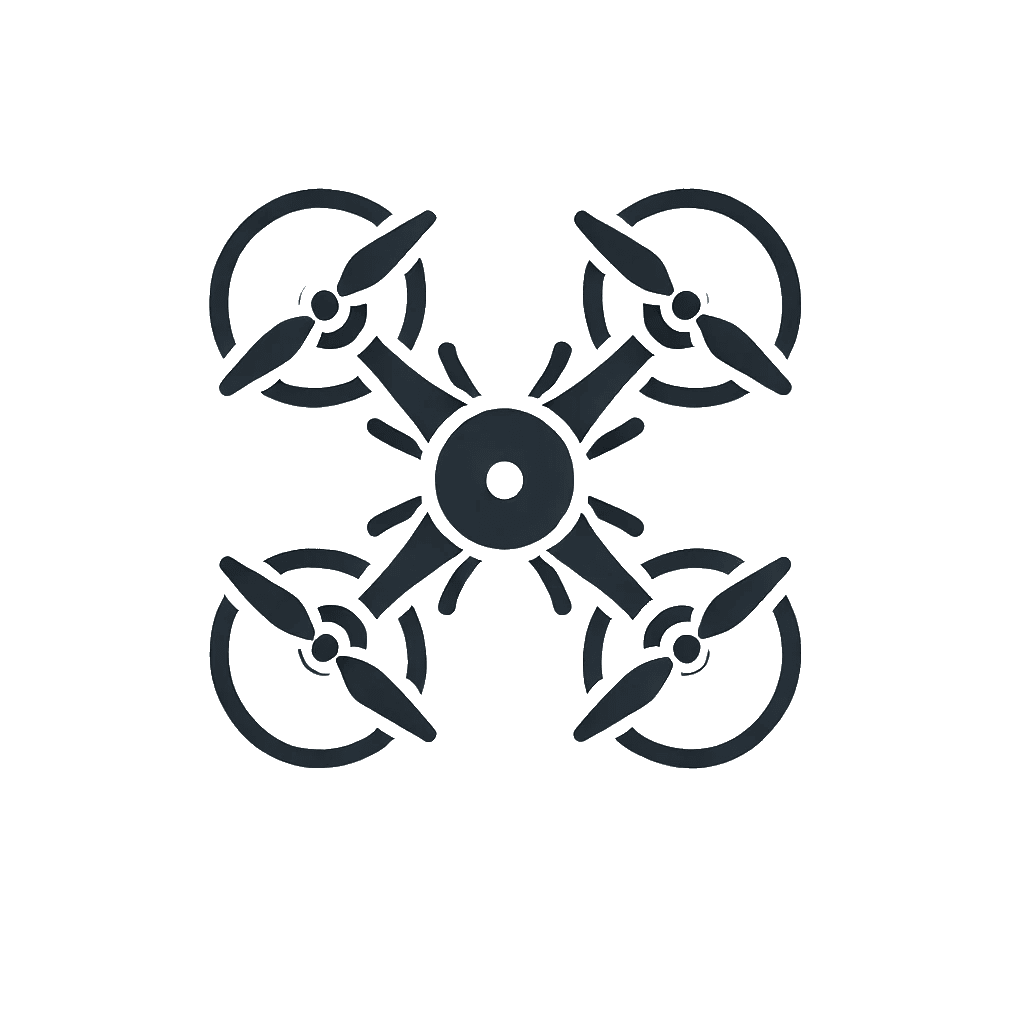
\includegraphics[width=1cm]{figures/drone_scheme.png}};
    \node[anchor=west] at (2,0.5) {\small drone};

    % Communication lines in legend
    \begin{scope}
        \draw[dotted] (4,0.5) -- (5,0.5);
        \node[anchor=west] at (5.1,0.5) {\small communication};
    \end{scope}
    
\end{tikzpicture}
    \caption{Illustration du scénario du 3e défi CAGE}\label{fig:cage_challenge}
\end{figure}

Le scénario met en scène trois types d'agents :
\begin{itemize}
    \item \textbf{Agents bleus (défenseurs)} : chargés de maintenir la sécurité et la fonctionnalité du réseau de drones. Leurs rôles consistent notamment à contrôler les drones, à empêcher tout accès non autorisé et à garantir l'intégrité des données. Ils peuvent effectuer des actions telles que \textit{RetakeControl}, \textit{RemoveOtherSessions} et \textit{BlockTraffic}.
    \item \textbf{Agents rouges (attaquants)} : visent à compromettre les drones afin de perturber la communication et le contrôle. Ils exploitent les vulnérabilités et peuvent effectuer des actions telles que \textit{ExploitDroneVulnerability}, \textit{SeizeControl} et \textit{FloodBandwidth}.
    \item \textbf{Agents verts (transfert de données)} : simulent des communications de données légitimes afin de tester l'intégrité du réseau, principalement à l'aide de l'action \textit{SendData}.
\end{itemize}

Chaque agent a une vision partielle de l'environnement, se concentrant sur des aspects tels que l'état du réseau, le statut des drones et les observations de communication. La structure de récompense des agents bleus est basée sur la réussite des transferts de données, le contrôle des drones, la sécurité du réseau et la gestion de la bande passante. Des récompenses positives sont accordées pour le maintien d'une communication sécurisée et fonctionnelle, tandis que des pénalités sont imposées pour les pertes de contrôle, les failles de sécurité et l'utilisation inefficace de la bande passante.

Ce défi souligne la nécessité de mesures de cybersécurité avancées, d'une gestion efficace des ressources et d'une coordination multi-agents efficace, ce qui en fait un banc d'essai pertinent pour le développement de CoPRAHOM.

\subsection{Modèles organisationnels}

\begin{figure*}[h!]
    \centering
    


\tikzset{every picture/.style={line width=0.75pt}} %set default line width to 0.75pt        

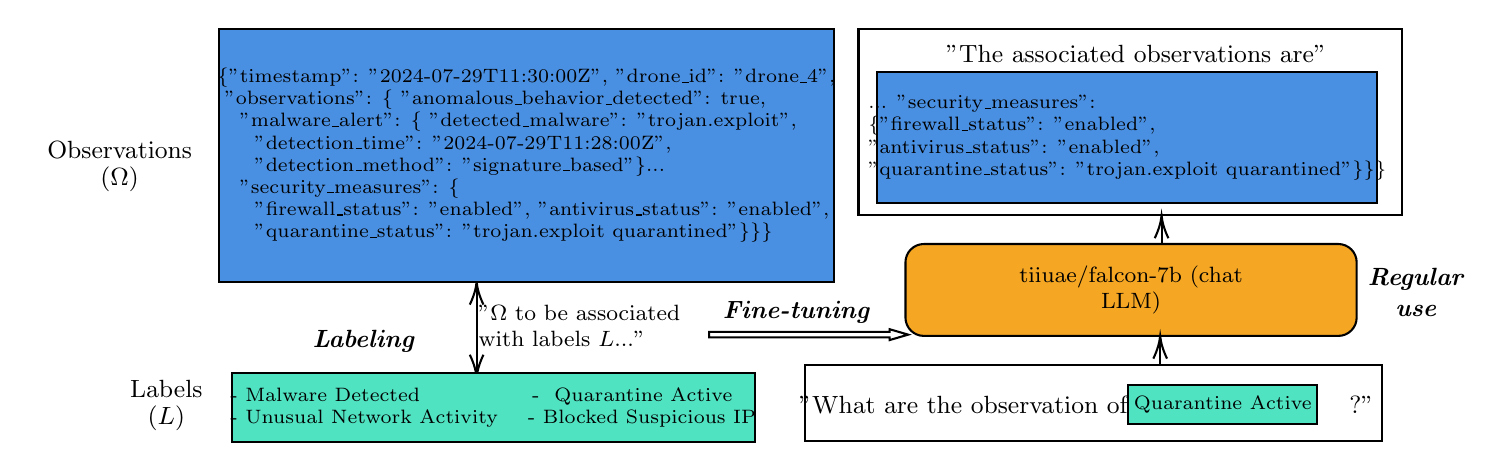
\begin{tikzpicture}[x=0.75pt,y=0.75pt,yscale=-1,xscale=1]
%uncomment if require: \path (0,1662); %set diagram left start at 0, and has height of 1662

%Rounded Rect [id:dp17386115134623514] 
\draw  [fill={rgb, 255:red, 245; green, 166; blue, 35 }  ,fill opacity=1 ] (424.61,402.58) .. controls (424.61,397.69) and (428.57,393.73) .. (433.46,393.73) -- (633.15,393.73) .. controls (638.04,393.73) and (642,397.69) .. (642,402.58) -- (642,429.15) .. controls (642,434.04) and (638.04,438) .. (633.15,438) -- (433.46,438) .. controls (428.57,438) and (424.61,434.04) .. (424.61,429.15) -- cycle ;
%Straight Lines [id:da8877910798706699] 
\draw    (547.33,451.83) -- (547.33,440) ;
\draw [shift={(547.33,438)}, rotate = 90] [color={rgb, 255:red, 0; green, 0; blue, 0 }  ][line width=0.75]    (10.93,-3.29) .. controls (6.95,-1.4) and (3.31,-0.3) .. (0,0) .. controls (3.31,0.3) and (6.95,1.4) .. (10.93,3.29)   ;
%Shape: Rectangle [id:dp44726237549140535] 
\draw   (376,452.18) -- (654,452.18) -- (654,488.66) -- (376,488.66) -- cycle ;
%Shape: Rectangle [id:dp2820683536345354] 
\draw   (402,290.27) -- (664,290.27) -- (664,379.64) -- (402,379.64) -- cycle ;
%Right Arrow [id:dp4162270206865013] 
\draw   (330,436.09) -- (417,436.09) -- (417,434.78) -- (425.91,437.39) -- (417,440) -- (417,438.7) -- (330,438.7) -- cycle ;
%Straight Lines [id:da8267677953106705] 
\draw    (548,393.83) -- (548,382) ;
\draw [shift={(548,380)}, rotate = 90] [color={rgb, 255:red, 0; green, 0; blue, 0 }  ][line width=0.75]    (10.93,-3.29) .. controls (6.95,-1.4) and (3.31,-0.3) .. (0,0) .. controls (3.31,0.3) and (6.95,1.4) .. (10.93,3.29)   ;
%Straight Lines [id:da6319519397458309] 
\draw    (218,456) -- (218,414) ;
\draw [shift={(218,412)}, rotate = 90] [color={rgb, 255:red, 0; green, 0; blue, 0 }  ][line width=0.75]    (10.93,-3.29) .. controls (6.95,-1.4) and (3.31,-0.3) .. (0,0) .. controls (3.31,0.3) and (6.95,1.4) .. (10.93,3.29)   ;
\draw [shift={(218,458)}, rotate = 270] [color={rgb, 255:red, 0; green, 0; blue, 0 }  ][line width=0.75]    (10.93,-3.29) .. controls (6.95,-1.4) and (3.31,-0.3) .. (0,0) .. controls (3.31,0.3) and (6.95,1.4) .. (10.93,3.29)   ;


% Text Node
\draw (68.5,471.5) node  [font=\footnotesize] [align=left] {\begin{minipage}[lt]{35.92pt}\setlength\topsep{0pt}
\begin{center}
{\small Labels ($\displaystyle L$)}
\end{center}

\end{minipage}};
% Text Node
\draw (372.5,426.5) node  [font=\small] [align=left] {\textit{\textbf{Fine-tuning}}};
% Text Node
\draw  [fill={rgb, 255:red, 74; green, 144; blue, 226 }  ,fill opacity=1 ]  (411,311) -- (652,311) -- (652,374) -- (411,374) -- cycle  ;
\draw (531.5,342.5) node  [font=\scriptsize] [align=left] {... "security\_measures":\\\{"firewall\_status": "enabled",\\"antivirus\_status": "enabled",\\"quarantine\_status": "trojan.exploit quarantined"\}\}\}};
% Text Node
\draw  [fill={rgb, 255:red, 80; green, 227; blue, 194 }  ,fill opacity=1 ]  (532,461.66) -- (623,461.66) -- (623,480.66) -- (532,480.66) -- cycle  ;
\draw (577.5,471.16) node  [font=\scriptsize] [align=left] {Quarantine Active};
% Text Node
\draw (536,302.25) node  [font=\footnotesize] [align=left] {{\small "The associated observations are"}};
% Text Node
\draw (671,417) node  [font=\small] [align=left] {\begin{minipage}[lt]{36.9pt}\setlength\topsep{0pt}
\begin{center}
\textit{\textbf{Regular}}\\\textit{\textbf{use}}
\end{center}

\end{minipage}};
% Text Node
\draw (512,471.16) node  [font=\footnotesize] [align=left] {{\small "What are the observation of \ \ \ \ \ \ \ \ \ \ \ \ \ \ \ \ \ \ \ \ \ \ \ \ \ ?"}};
% Text Node
\draw (46,356.32) node  [font=\footnotesize] [align=left] {\begin{minipage}[lt]{59.79pt}\setlength\topsep{0pt}
\begin{center}
{\small Observations ($\displaystyle \Omega $)}
\end{center}

\end{minipage}};
% Text Node
\draw (164,440.5) node  [font=\small] [align=left] {\textit{\textbf{Labeling}}};
% Text Node
\draw (267.5,433) node  [font=\footnotesize] [align=left] {{\footnotesize "$\displaystyle \Omega $ to be associated}\\{\footnotesize with labels $\displaystyle L$..."}};
% Text Node
\draw (533.3,415.86) node  [font=\footnotesize] [align=left] {\begin{minipage}[lt]{99.33pt}\setlength\topsep{0pt}
\begin{center}
tiiuae/falcon-7b (chat LLM)
\end{center}

\end{minipage}};
% Text Node
\draw  [fill={rgb, 255:red, 80; green, 227; blue, 194 }  ,fill opacity=1 ]  (100,456) -- (352,456) -- (352,489) -- (100,489) -- cycle  ;
\draw (226,472.5) node  [font=\scriptsize] [align=left] {\mbox{-} Malware Detected \ \ \ \ \ \ \ \ \ \ \ \ \ \ - \ Quarantine Active\\\mbox{-} Unusual Network Activity \ \ \ - Blocked Suspicious IP};
% Text Node
\draw  [fill={rgb, 255:red, 74; green, 144; blue, 226 }  ,fill opacity=1 ]  (94,290) -- (390,290) -- (390,412) -- (94,412) -- cycle  ;
\draw (242,351) node  [font=\scriptsize] [align=left] {\{"timestamp": "2024-07-29T11:30:00Z", "drone\_id": "drone\_4",\\ \ "observations": \{ "anomalous\_behavior\_detected": true,\\ \ \ \ "malware\_alert": \{ "detected\_malware": "trojan.exploit",\\ \ \ \ \ \ "detection\_time": "2024-07-29T11:28:00Z",\\ \ \ \ \ \ "detection\_method": "signature\_based"\}...\\ \ \ \ "security\_measures": \{\\ \ \ \ \ \ "firewall\_status": "enabled", "antivirus\_status": "enabled",\\ \ \ \ \ \ "quarantine\_status": "trojan.exploit quarantined"\}\}\}};


\end{tikzpicture}
    \caption{Formation et utilisation du LLM pour l'application du CoPRAHOM au 3e défi CAGE}\label{fig:llm_process}
\end{figure*}


Nous avons mis en œuvre et évalué deux modèles organisationnels à l'aide du modèle \textit{MASCARA-$\mathcal{M}OISE^+$} et adaptés à l'environnement du 3e défi CAGE de CybORG :

Le modèle « \textbf{Active Defense} » met en œuvre des mesures proactives pour anticiper, détecter et atténuer les menaces. Il vise à maintenir la sécurité et la fonctionnalité du réseau grâce à trois rôles prédéfinis :
%
\textit{Évaluateur des menaces} : surveille le réseau et identifie les menaces potentielles à l'aide d'analyses avancées ;
\textit{Stratège en réponse} : supervise les stratégies de réponse visant à neutraliser les menaces identifiées ;
\textit{Gardien du réseau} : garantit l'intégrité et la disponibilité du réseau en mettant en œuvre des mesures de sécurité.
%
Ce modèle comprend également la mission « Détection proactive des menaces », qui comprend des objectifs de détection précoce des menaces à l'aide d'analyses prédictives.

La « \textbf{Isolation des éléments suspects} » met l'accent sur l'identification et l'isolation des éléments compromis du réseau afin de contenir les menaces grâce à trois rôles :
%
\textit{Détecteur d'anomalies} : identifie les anomalies indiquant des violations potentielles ;
\textit{Spécialiste de l'isolation} : isole les systèmes compromis afin d'empêcher la propagation des menaces ;
\textit{Intervenant en cas d'incident} : coordonne la réponse et exécute les protocoles d'isolement.
%
Ce modèle comprend également la mission \textit{Détection des drones compromis}, qui comprend des objectifs visant à détecter les drones compromis et à les isoler du réseau, ainsi que la mission \textit{Confinement et isolation}, qui comprend des objectifs visant à isoler les systèmes compromis du réseau.

De plus, nous avons établi un modèle non basé sur MASCARA appelé « \textbf{Manuel} » à partir de notre compréhension empirique de l'environnement, qui sert de modèle de référence.
Nous avons également pris en compte un cas totalement sans contrainte, appelé « \textbf{Libre} », qui sert de référence MARL standard à des fins de comparaison.


\subsection{Procédure expérimentale}

Nous avons formé chaque modèle organisationnel à l'aide du \textit{CoPRAHOM Wrapper} avec le simulateur \textit{CybORG} fourni. Le wrapper intègre les spécifications et les contraintes organisationnelles pendant l'apprentissage, permettant aux agents d'apprendre et d'adapter leur comportement en fonction de rôles et de missions prédéfinis.

Nous avons sélectionné l'algorithme MAPPO pour son efficacité éprouvée dans des environnements multi-agents coopératifs sans nécessiter de modifications algorithmiques ou d'architectures spécifiques au domaine~\cite{Yu2022}. Nous avons utilisé le modèle d'algorithme implémenté MAPPO fourni par MARLlib. Plus précisément, nous avons configuré le modèle MAPPO avec un réseau MLP à deux couches, comprenant 128 neurones dans la première couche et 256 dans la seconde, optimisé à l'aide d'Adam avec un taux d'apprentissage de 0,0003. Ces configurations ont été choisies sur la base d'expériences préliminaires et des modèles d'hyperparamètres affinés disponibles dans MARLlib. Nous avons lancé l'entraînement sur 70 itérations (chacune comprenant 128 épisodes) selon un mode d'apprentissage centralisé et d'exécution décentralisée.\\

Pour former le LLM avec \texttt{ol\_mngr}, nous avons exploré l'environnement manuellement, étape par étape, à l'aide de politiques contrôlées. Cette approche a permis à l'agent de rencontrer les situations les plus pertinentes pour détecter et atténuer les programmes malveillants. Il s'agit par exemple de situations dans lesquelles un agent reçoit des messages que nous jugeons suspects ou dans lesquelles un agent reçoit la confirmation de tuer un processus. Tout au long de cette exploration, nous avons collecté, affiché (sous forme de JSON ou de graphique), interprété et étiqueté plusieurs observations à l'aide de quelques mots-clés. Cet étiquetage permet d'identifier facilement les comportements collectifs sur la base d'observations visuelles, ce qui permet de mieux contrôler les actions des agents. L'ensemble du processus de formation et d'utilisation est résumé dans \autoref{fig:llm_process}.

\subsection{Mesures d'évaluation}

Nous avons utilisé divers indicateurs pour mesurer l'impact de CoPRAHOM pendant et après la formation :
\begin{itemize}
    \item \textbf{Évolutivité} : évalue la capacité à gérer un nombre croissant d'agents et d'obstacles en fonction de l'utilisation des ressources informatiques.
    \item \textbf{Temps de convergence} : nombre d'épisodes nécessaires à l'algorithme pour atteindre une solution stable. Des temps de convergence plus courts indiquent un apprentissage plus rapide.
    \item \textbf{Écart type} : indique la variabilité des récompenses obtenues par les agents. Un écart type plus faible signifie des performances plus régulières et une organisation potentiellement plus stable.
    \item \textbf{Récompense moyenne} : La récompense moyenne obtenue par épisode reflète la performance globale de l'algorithme.
    \item \textbf{Respect des contraintes} : Évalue dans quelle mesure les agents respectent les contraintes organisationnelles données. %Il est calculé comme l'inverse du nombre de fois où les contraintes ne sont pas respectées. Un respect élevé des contraintes signifie que les agents suivent efficacement les règles.
\end{itemize}

Nous avons également inclus ces deux indicateurs spécifiques à la cyberdéfense :
\begin{itemize}
    \item \textbf{Pourcentage moyen de drones infectés par des logiciels malveillants} : mesure la proportion de drones infectés par des logiciels malveillants pendant la simulation.
    \item \textbf{Pourcentage moyen d'attaques de logiciels malveillants réussies} : indique le taux de réussite des attaques contre l'essaim de drones.
\end{itemize}

\subsection{Critères de validation}

À l'aide des indicateurs susmentionnés, nous avons défini des critères pour évaluer l'amélioration de la cyberdéfense fournie par CoPRAHOM par rapport à l'apprentissage MARL classique, en mettant particulièrement l'accent sur le modèle « défense active ». Ces critères sont les suivants :

\begin{itemize}
    \item $\mathbf{C_1}$ : Nous nous attendons à observer manuellement certaines stratégies collectives, telles que l'isolation des activités suspectes ou la coordination des manœuvres défensives.
    \item $\mathbf{C_2}$ : Nous nous attendons à une convergence plus rapide dans les modèles « Active Defense » ou « Suspect Isolation » que dans le cas « Free », et à une courbe d'apprentissage constante dans le cas « Manual ».
    \item $\mathbf{C_3}$ : Nous nous attendons à des récompenses plus élevées dans les modèles « Active Defense » ou « Suspect Isolation » par rapport au cas « Free ».
    \item $\mathbf{C_{4}}$ : Nous nous attendons à ce que l'écart type diminue entre les modèles « Libre » et « Défense active » ou « Isolation des suspects », puis entre les modèles « Défense active » ou « Isolation des suspects » et le modèle « Manuel », car les agents sont de plus en plus contraints dans leur comportement.
    \item $\mathbf{C_{5}}$ : Nous nous attendons à ce que le respect des contraintes soit entièrement couvert dans les modes \textit{correct} et \textit{correct\_policy}, mais pas dans le mode \textit{penalize}.
    \item $\mathbf{C_{6}}$ : Nous nous attendons à ce que l'évolutivité soit gérée dans tous les cas.
    \item $\mathbf{C_7}$ : Pourcentage moyen inférieur de drones infectés dans les modèles « Active Defense » ou « Suspect Isolation » par rapport au cas « Free ».
    \item $\mathbf{C_8}$ : Pourcentage moyen d'attaques de logiciels malveillants réussies inférieur dans les modèles « Active Defense » ou « Suspect Isolation » par rapport au cas « Free ».

\end{itemize}

\section{Résultats et discussion}\label{sec:results_and_discussion}

\autoref{fig:learning_curves} illustre les courbes d'apprentissage des modèles « Suspect Isolation », « Active Defensive » et « Manual », indiquant leurs taux de convergence au cours des épisodes d'entraînement.
\autoref{tab:metrics_comparison} résume le temps de convergence pendant l'entraînement ainsi que les récompenses moyennes, l'écart type, le nombre moyen de drones infectés et le nombre moyen d'attaques de logiciels malveillants obtenus par les modèles après une douzaine d'épisodes d'entraînement.

\begin{figure}[ht]
    \centering
    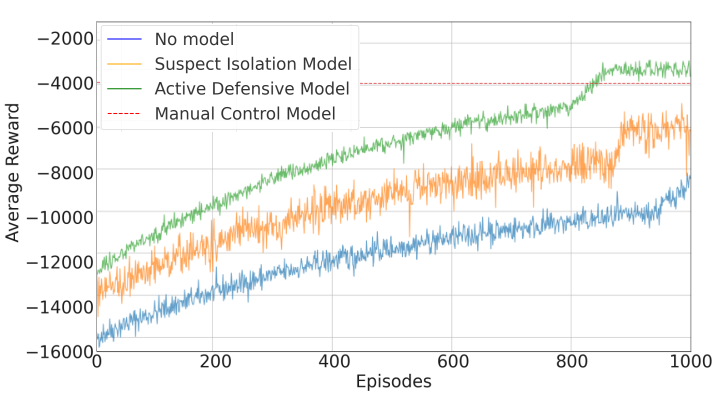
\includegraphics[width=1\linewidth]{figures/learning_curves.png}
    \caption{Courbes d'apprentissage pour \textit{Gratuit}, \textit{Isolation suspecte}, \textit{Défense active}, \textit{Manuel} en utilisant le mode \textit{correct\_policy} }
    \label{fig:learning_curves}
\end{figure}

\begin{table*}[t]
    \centering
    \setlength{\tabcolsep}{4.5pt}
    \caption{Comparaison des modèles et des modes de contrainte par rapport aux métriques.}
    \label{tab:metrics_comparison}
    \begin{tabular}{lcccccccccccc}
                                                         & {Gratuit}   & \multicolumn{3}{c}{Isolation des suspects} & \multicolumn{3}{c}{Défense active} & {Manuel}                                                                                     \\
        % \cline{2-13}
        Métrique                                         &             & Pénaliser                                  & Corriger                           & Corriger\_Politique & Pénaliser & Corriger & Corriger\_Politique &                           \\
        \midrule
        Récompense moyenne                               & -8727,49    & -5900,00                                   & -6085,12                           & -6088,00            & -3055,36  & -3100,00 & -3060,00            & -3906,00                  \\
        Écart type                                       & 138,00      & 2148,0                                     & 2027,0                             & 2018,00             & 962,      & 940,00   & 945,00              & 570,33                    \\
        Évolutivité                                      & Moyenne     & Élevée                                     & Moyenne                            & Moyenne             & Élevée    & Moyenne  & Moyenne             & Moyenne                   \\
        Temps de convergence                             &             & gt;1000                                    & 1000                               & 950                 & 950       & 800      & 850                 & 850         & $\emptyset$ \\
        Respect des contraintes                          & $\emptyset$ & Faible                                     & Élevé                              & Élevé               & Moyen     & Élevé    & Élevé               & $\emptyset$               \\
        Moyenne inf. drones (\%)                         & 61,0        & 43,0                                       & 30,0                               & 23,0                & 24,0      & 25,0     & 20,0                & 40,0                      \\
        Attaques de logiciels malveillants moyennes (\%) & 72,0        & 55,0                                       & 52,0                               & 45,0                & 38,0      & 45,0     & 40,0                & 51,0                      \\
    \end{tabular}
\end{table*}

Les modèles organisationnels ont efficacement influencé le comportement des drones dans l'environnement CybORG CAGE Challenge 3. Le modèle « Suspect Isolation » (isolement des suspects) a démontré son efficacité dans l'identification et l'isolement des drones présentant des activités suspectes, renforçant ainsi la sécurité globale. Ce modèle a permis d'identifier et de neutraliser rapidement les menaces potentielles, empêchant ainsi la propagation d'activités malveillantes au sein du essaim de drones ($\mathbf{C_1}$).

\autoref{fig:learning_curves} fournit une vue d'ensemble des courbes d'apprentissage pour chaque modèle. Le modèle « Free » (bleu) a présenté la convergence la plus lente et les récompenses moyennes les plus faibles. De plus, il montre également une faible variabilité des récompenses, ce qui indique que les agents sont lentement formés avec des changements limités à chaque étape. Ce résultat est prévisible, car le taux d'apprentissage pour MAPPO est relativement faible.

En revanche, le modèle « Suspect Isolation » (orange) a montré une convergence plus rapide et des récompenses moyennes plus élevées que le modèle « Free ». Cependant, la variabilité accrue (par rapport au modèle « Free ») suggère que, comme les agents sont contraints/incités à respecter certaines règles pour identifier et isoler les activités suspectes, leurs politiques peuvent nécessiter un certain temps pour s'habituer à ces règles et atteindre un comportement plus stable.

Le modèle « Active Defense » (vert) a affiché les récompenses moyennes les plus élevées et la convergence la plus rapide parmi tous les modèles. L'augmentation constante des récompenses démontre l'efficacité des stratégies de défense proactive mises en œuvre par les agents. Ce modèle a montré la plus grande amélioration des performances, soulignant les avantages de l'utilisation de contraintes organisationnelles structurées pour guider le comportement des agents. Le modèle « Active Defense » présente également une variabilité des récompenses plus faible que le modèle « Suspect Isolation », mais plus élevée que le modèle « Free ». Cela suggère que, même si les agents sont encore en phase d'adaptation aux contraintes, leurs comportements possibles sont plus limités dans le modèle « Active Defense » que dans le modèle « Suspect Isolation ».

Le modèle « Manuel » (ligne rouge en pointillés) a servi de référence pour la comparaison. Il a obtenu de meilleurs résultats que les modèles « Libre » et « Isolation des suspects », mais a été surpassé par le modèle « Défense active ». Cela s'explique par le fait que la stratégie de contrôle manuel, bien qu'efficace, manquait de l'adaptabilité et de l'efficacité fournies par les modèles organisationnels appris.

D'un point de vue quantitatif, les mesures fournissent également des preuves des avantages liés à l'application de contraintes organisationnelles. Comme l'illustre la figure \autoref{fig:learning_curves}, dans le cas d'une politique contrainte, les agents ont convergé plus rapidement que dans le modèle « Libre » dans tous les modes. Cela confirme que les contraintes organisationnelles peuvent accélérer l'apprentissage ($\mathbf{C_2}$). Comme prévu, la politique élaborée manuellement a permis une convergence immédiate, en raison de l'absence d'apprentissage.

Les mesures de récompense moyenne révèlent que les agents guidés par le modèle « Suspect Isolation » ont systématiquement surpassé ceux du modèle « Free », obtenant des récompenses plus élevées ($\mathbf{C_3}$). Cela indique que les contraintes organisationnelles améliorent non seulement l'efficacité de l'apprentissage, mais aussi les performances globales. Les politiques élaborées manuellement ont systématiquement obtenu les récompenses les plus élevées, soulignant l'efficacité de contraintes bien définies.

En ce qui concerne les modèles contraints, l'écart type dans \autoref{tab:metrics_comparison} a diminué progressivement du modèle le moins contraint, tel que « Suspect Isolation », au modèle le plus contraint, tel que « Active Defense » ($\mathbf{C_4}$). Cette réduction de la variabilité suggère que les contraintes organisationnelles contribuent à un comportement plus stable et plus cohérent des agents.

Le critère de respect des contraintes a été pleinement satisfait dans les modes \textit{correct} et \textit{correct\_policy}, mais pas dans le mode \textit{penalize} ($\mathbf{C_5}$). Cela démontre que si les agents peuvent apprendre à respecter efficacement les contraintes, le mode d'intégration des contraintes joue un rôle crucial. Dans notre évaluation, les modes « correct » et « correct\_policy » ont démontré une adhésion totale aux contraintes organisationnelles, comme en témoigne l'absence totale de déviations dans le comportement des agents par rapport aux rôles et missions prescrits. En revanche, le mode « pénaliser » a montré des déviations occasionnelles, en particulier dans les modèles peu contraints tels que « Suspect Isolation ». Cela suggère que les agents privilégient parfois la maximisation des récompenses plutôt que le respect strict des contraintes. Une analyse plus approfondie des stratégies de pénalisation permettrait d'améliorer la conformité.

L'évolutivité, évaluée en analysant les performances du système lorsque le nombre d'agents et d'obstacles augmente, a été gérée efficacement dans tous les modèles ($\mathbf{C_6}$). En particulier, le mode \textit{penalize} a montré une évolutivité supérieure grâce à un calcul efficace intégré des mises à jour des politiques, contrairement aux modes \textit{correct} et \textit{correct\_policy} qui nécessitent des fonctions de correction supplémentaires.

Les modèles « Active Defense » et « Suspect Isolation » ont tous deux eu un impact sur les indicateurs « Pourcentage moyen de drones infectés » et « Pourcentage moyen d'attaques de logiciels malveillants réussies » ($\mathbf{C_7}$ et $\mathbf{C_8}$). Cependant, il est important de noter que ces deux indicateurs ne sont pas directement liés à la récompense globale, car ils sont calculés séparément. Le modèle « Active Defense » a obtenu les meilleurs résultats, réduisant le pourcentage de drones infectés à 23 % et le taux de réussite des attaques de logiciels malveillants à 38 %. Cette réduction significative, comparée au taux d'infection de 61 % et au taux de réussite de 72 % du modèle « Free », démontre l'efficacité des stratégies défensives proactives dans la prévention de la propagation des logiciels malveillants et des attaques réussies. Le modèle « Isolation des suspects » a également affiché des taux d'infection et de réussite des attaques inférieurs à ceux du modèle « Libre ».

% Ces résultats soulignent l'importance de mettre en œuvre des contraintes organisationnelles structurées et des mécanismes de défense proactifs au sein des systèmes autonomes. L'intégration des modèles organisationnels $\mathcal{M}OISE^+$ dans le cadre MARL, comme le démontre CoPRAHOM, améliore considérablement l'efficacité et la coordination des agents de cyberdéfense autonomes. Les résultats expérimentaux soulignent que les contraintes organisationnelles structurées améliorent non seulement les performances et la stabilité des agents, mais garantissent également que leur comportement est conforme aux objectifs de la mission et aux objectifs de cybersécurité.

% Les résultats suggèrent qu'un affinement des spécifications organisationnelles et l'intégration de règles et de protocoles plus sophistiqués pourraient améliorer encore davantage le comportement et la coordination des agents. Ce développement continu promet de renforcer la résilience et la robustesse des stratégies de cyberdéfense face à des menaces de plus en plus sophistiquées.
% Cependant, la généralisation de CoPRAHOM à différents scénarios de cyberdéfense réels, tels que la sécurité de l'IoT ou les systèmes de contrôle industriel, pourrait nécessiter des ajustements des spécifications organisationnelles et des contraintes politiques. Les travaux futurs devraient explorer ces adaptations afin de valider la large applicabilité de CoPRAHOM.

\section{Conclusion}\label{sec:conclusion}

Notre contribution est motivée par le coût élevé de la conception de systèmes multi-agents de cyberdéfense (MAS) dans divers scénarios, en particulier lorsqu'il s'agit de faire face à des menaces en constante évolution. Pour remédier à ce problème, nous proposons un algorithme dédié appelé CoPRAHOM, qui exploite l'apprentissage par renforcement multi-agents (MARL) en fonction des spécifications organisationnelles. CoPRAHOM garantit le respect de certaines contraintes dans le comportement des agents, ce qui facilite la surveillance et la compréhension des agents formés.

CoPRAHOM a été évalué à l'aide de notre implémentation PoC proposée pour le 3e défi CAGE, un scénario coopératif de cyberdéfense par essaim de drones conçu pour limiter/éliminer les programmes malveillants et leur impact. Nous avons établi divers modèles organisationnels, allant de modèles minimalement contraints à des modèles entièrement contraints. Nous avons évalué les stratégies collectives émergentes, affinées ou prédéfinies sur la base de critères de performance pendant et après la formation.

Les résultats indiquent que les modèles équilibrés en termes de contraintes, tels que le « modèle défensif actif », permettent d'obtenir un compromis significatif entre les contraintes et l'apprentissage autonome. Ce modèle utilise des règles prédéfinies simples pour détecter et traiter les menaces lorsque les observations sont sans ambiguïté, tout en permettant à l'agent d'apprendre à réagir dans d'autres scénarios.

Outre la contrainte des agents en fonction des spécifications organisationnelles, nous souhaitons prendre en compte des mécanismes d'explicabilité afin de comprendre les nouveaux modèles organisationnels appris. L'idée d'une amélioration itérative entre l'entraînement et l'explicabilité pourrait grandement bénéficier de l'apprentissage hiérarchique, qui aide à caractériser et à mettre en évidence les stratégies pendant l'apprentissage.
%En outre, si les premiers résultats obtenus avec LLM montrent qu'il s'agit d'un outil complémentaire prometteur pour CoPRAHOM, il pourrait également offrir de nouvelles pistes pour expliquer les comportements collectifs, en particulier dans les scénarios de cyberdéfense où la plupart des environnements en réseau ne sont pas représentables de manière visuelle ou intuitive.

% Enfin, nous visons également à améliorer l'applicabilité de PRAHOM en développant des interfaces dédiées autour de PRAHOM afin de le rendre plus accessible aux contextes industriels et de recherche.
